\label{chap:results}
\begin{table*}[]
\centering
\caption{Summary of results for \texttt{bmi\_refresh}, \texttt{static\_batch},
    \texttt{partial\_refresh} and \texttt{precision\_strategy}}
\label{table.summary}
\resizebox{\textwidth}{!}{%
\begin{tabular}{|c|c|c|c|c|c|}
\hline
\textbf{Strategy} & \begin{tabular}[x]{@{}c@{}}
    \textbf{Avg. Recall}\\ \textbf{@($E_{norm}$=1)}
\end{tabular} & \begin{tabular}[x]{@{}c@{}}
\textbf{Avg. Recall}\\ \textbf{@($E_{norm}$=1.5)}
\end{tabular} & \begin{tabular}[x]{@{}c@{}}
\textbf{Avg. Recall}\\ \textbf{@($E_{norm}$=2)}
\end{tabular} & \begin{tabular}[x]{@{}c@{}}
\textbf{$E_{norm}$ for}\\ \textbf{75\% recall}
\end{tabular}&
\begin{tabular}[x]{@{}c@{}}
    \textbf{Running Time}\\ \textbf{(in min)}
\end{tabular} \\ \hline \hline
\texttt{exponential} & 0.723 & 0.832 & 0.887 & 2.160 & 0.33 \\ \hline \hline
\texttt{static(k=1)} & 0.754 & 0.856 & 0.900 & 1.997 & 34.19 \\ \hline
\texttt{static(k=100)} & 0.652 & 0.769 & 0.840 & 2.461 & 0.34 \\ \hline
\hline
\texttt{partial(k=10,s=1000)} & 0.753 & 0.855 & 0.899 & 1.993 & 18.22 \\ \hline
\texttt{partial(k=100,s=500)} & 0.731 & 0.839 & 0.893 & 2.032 & 16.50 \\ \hline
\texttt{partial(k=100,s=1000)} & 0.737 & 0.844 & 0.893 & 2.025 & 16.57 \\ \hline
\texttt{partial(k=100,s=5000)} & 0.747 & 0.852 & 0.896 & 1.982 & 17.34 \\ \hline
\texttt{partial(k=500,s=1000)} & 0.686 & 0.770 & 0.804 & 2.812 & 16.09 \\ \hline
\hline
\texttt{precision(p=0.4,m=25)} & 0.679 & 0.844 & 0.892 & 2.116 & 17.63 \\ \hline
\texttt{precision(p=0.6,m=25)} & 0.728 & 0.853 & 0.897 & 2.096 & 20.22 \\ \hline
\texttt{precision(p=0.8,m=25)} & 0.749 & 0.855 & 0.900 & 2.024 & 20.24 \\ \hline
\texttt{precision(p=1.0,m=25)} & 0.755 & 0.855 & 0.900 & 1.992 & 21.02 \\ \hline
\end{tabular}
}
\end{table*}
In this chapter, we dive into the results of our experiments and compare
all the refresh strategies.

For sake of readability, we encode each strategy with their parameter
settings as \texttt{strategy\_name(param1=x,$\ldots$)}. For reference, Table~\ref{table.strategies}
lists all the strategies and their parameters.
We summarize the average results obtained across all the datasets for different
parameter settings of \texttt{exponential}, \texttt{static},
\texttt{partial} and \texttt{precision} in Table~\ref{table.summary}.
Table~\ref{table.summary_athome1},~\ref{table.summary_athome2},~\ref{table.summary_athome3}
and~\ref{table.summary_athome4} reports the dataset-level results obtained when
using \texttt{athome1}, \texttt{athome2}, \texttt{athome3} and \texttt{athome4}
, respectively.
In these tables, we report the recall achieved at certain values of effort, effort required to
achieve $75\%$ recall, and the average running time. Instead of absolute effort,
we use normalized effort $E_{norm}$ as defined in Section~\ref{sec:eval}. For
example, ``Avg. recall@($E_{norm}=1.5$)'' refers to the average recall achieved
across all the topics when $1.5 \times R$ documents haven been assessed, where $R$
is the total number of relevant documents for a topic.

\subsection*{Static Batch Refresh Strategy}
Figure~\ref{plot:bmi_static} compares the gain curves for \texttt{exponential},
\texttt{static(k=1)} and \texttt{static(k=100)}.

With \texttt{static(k=1)}, CAL achieves noticeably higher recall of
$0.754$ at $E_{norm} = 1$ than \texttt{exponential} which achieves $0.723$
recall.  \texttt{static(k=100)} performs worse than
\texttt{exponential}, managing to achieve $0.652$ recall at the same effort.
These results establish that frequent refreshing improves the effectiveness of a
CAL system.
Although the batch sizes in BMI increases exponentially with time, it still does
frequent refreshes during the early stages of the CAL process, thus performing
better than \texttt{static(k = 100)}. \texttt{exponential} is also
extremely cheap in terms of total computation cost since it only performs a
logarithmic number of refreshes compared to the \texttt{static} strategies.
The \texttt{exponential} simulation finished in less than a minute while
\texttt{static(k=1)} took little more than a half hour.

Using Student's paired t-test, we found that \texttt{static(k=1)} was
significantly better than \texttt{exponential} in terms of recall achieved at
$E_{norm} \in \{1,1.5\}$ ($p < 0.05$ for \texttt{athome1} and \texttt{athome3},
$p < 0.0001$ for \texttt{athome4}). However, for the \texttt{athome2}
collection, the improvement was negligible. When $E_{norm} = 2$, the difference
in recall achieved by both the strategies are insignificant for \texttt{athome1}
and \texttt{athome3} ($p > 0.1$). As evident from the gain curve in
Figure~\ref{plot:bmi_static}, the recall values at $E_{norm} = 2$ plateaus
at a high value for these strategies.

We evaluate rest of the refresh strategies by comparing them to
\texttt{static(k = 1)}.

\begin{figure}
    \centering
    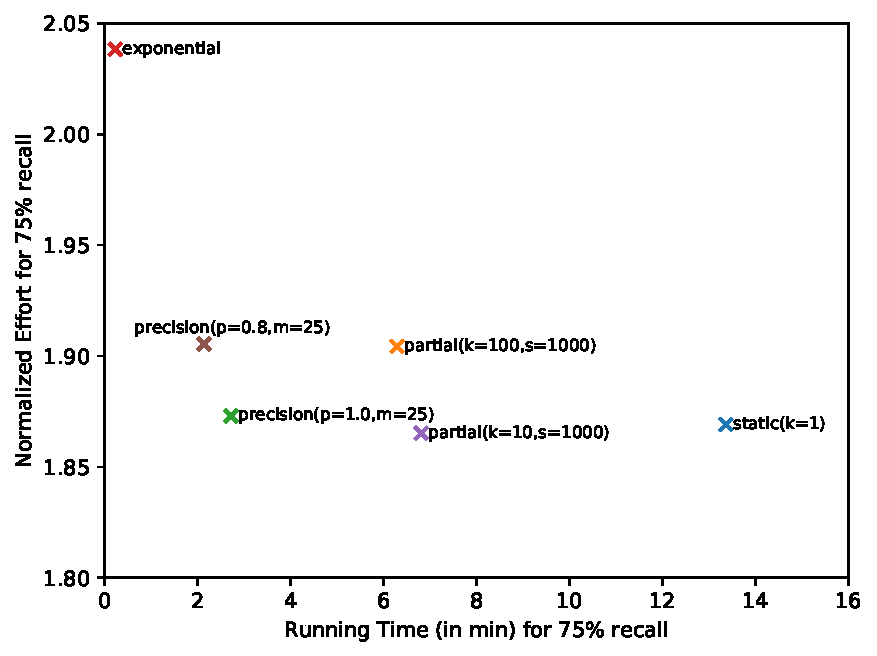
\includegraphics[width=0.7\textwidth]{plots/eff_vs_eff.pdf}
    \caption{Effectiveness vs Efficiency plot for selected refresh strategies}
    \label{plot:eff_vs_eff}
\end{figure}

\subsection*{Partial Refresh Strategy}
Figure~\ref{plot:partial1} compares the gain curves for
\texttt{static(k=1)}, \texttt{partial(k=100,s=1000)} and
\texttt{partial(k=500,s=1000)}.

By fixing the partial set size \texttt{s=1000} and varying the full refresh
period \texttt{k} in \texttt{partial}, we observe
that for \texttt{k=10} and \texttt{k=100}, the difference in recall remains insignificant throughout the
CAL process. Their recall values are also very similar to
\texttt{static(k=1)}. They achieve $0.855$ and $0.844$ recall, respectively at
$E_{norm} = 1.5$. For \texttt{k=500}, we observe $0.770$ recall at the
same effort, which is worse than \texttt{exponential} ($0.832$). This is in
agreement with our previous observation that more frequent full refreshes
increases CAL's effectiveness. \texttt{static(k=100)}
consistently achieved lower recall when compared to \texttt{static(k=1)} while
\texttt{partial(k=100,s=1000)} is much closer to the latter. Based
on this, it can be established that partial refreshing contributes noticeable
improvements to recall over plain static batch refreshing with same 
frequency of full refresh.

Figure~\ref{plot:partial2} shows the effect of varying partial set size
\texttt{s} when the full refresh period \texttt{k} is fixed to $100$. We observe
no changes to the recall values when the size of partial set is 500 or higher. At
$s=100$, the decrease in performance is noticeable.

\texttt{partial} simulations on average ran $50.44\%$ faster than
\texttt{static(k=1)}. While achieving similar effectiveness as 
\texttt{static(k=1)}, \texttt{partial(k=10,s=1000)} ran $46.71\%$ faster.

\texttt{partial(k=10,s=1000)} was the optimal setting across all our
experiments.  For any dataset, there was no significant difference ($p > 0.1$)
between the recall achieved by \texttt{partial(k=10,s=1000)} and
\texttt{static(k=1)} at $E_{norm} \in \{1,1.5,2\}$. For \texttt{athome1}, even
\texttt{partial(k=100,s=1000)} was an optimal setting as there was no
significant difference ($p > 0.45$) between the recall achieved by
\texttt{partial(k=100,s=1000)} and \texttt{partial(k=10,s=1000)} at $E_{norm}
\in \{1,1.5,2\}$.

\begin{figure}
    \centering
    \begin{subfigure}[t]{0.48\textwidth}
        \centering
        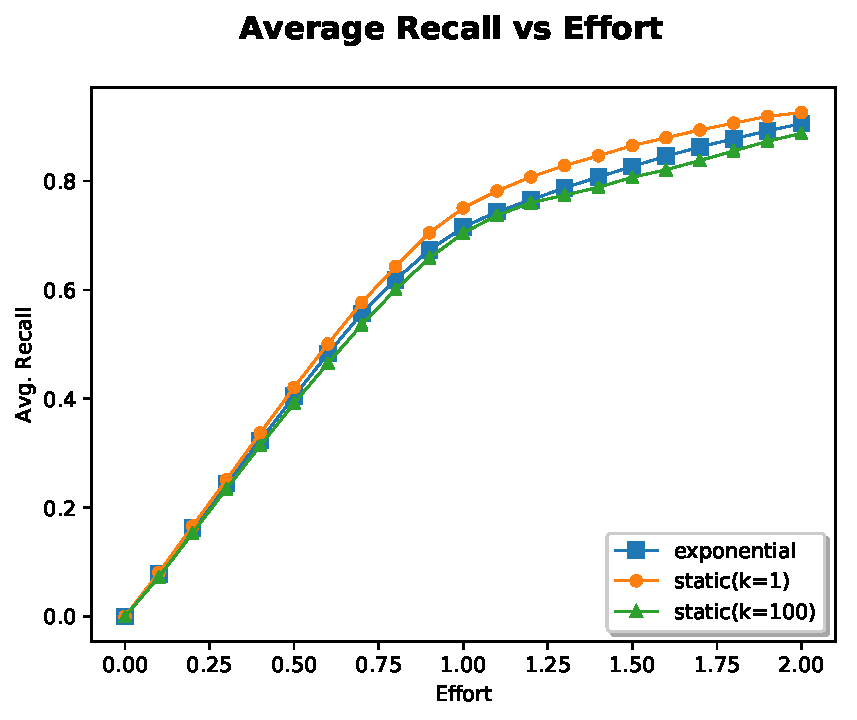
\includegraphics[width=\textwidth]{plots/bmi_static.pdf}
        \caption{Comparison of \texttt{exponential} and \texttt{static}.
            \texttt{static(k=1)} consistently outperforms the rest.}
        \label{plot:bmi_static}
    \end{subfigure}
    ~
    \begin{subfigure}[t]{0.48\textwidth}
        \centering
        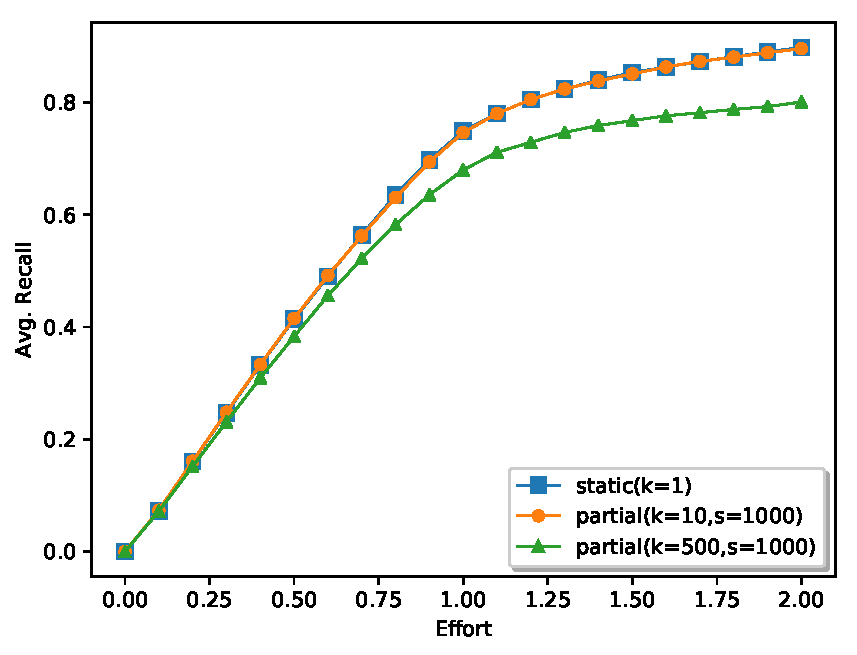
\includegraphics[width=\textwidth]{plots/static_partial.pdf}
        \caption{Comparison of \texttt{partial} and \texttt{static(k=1)}. We fix
            the partial set size to 1000 and observe that
            \texttt{partial(k=10,s=1000)} performs very similar to
        \texttt{static(k=1)}.}
        \label{plot:partial1}
    \end{subfigure}

    \begin{subfigure}[t]{0.48\textwidth}
        \centering
        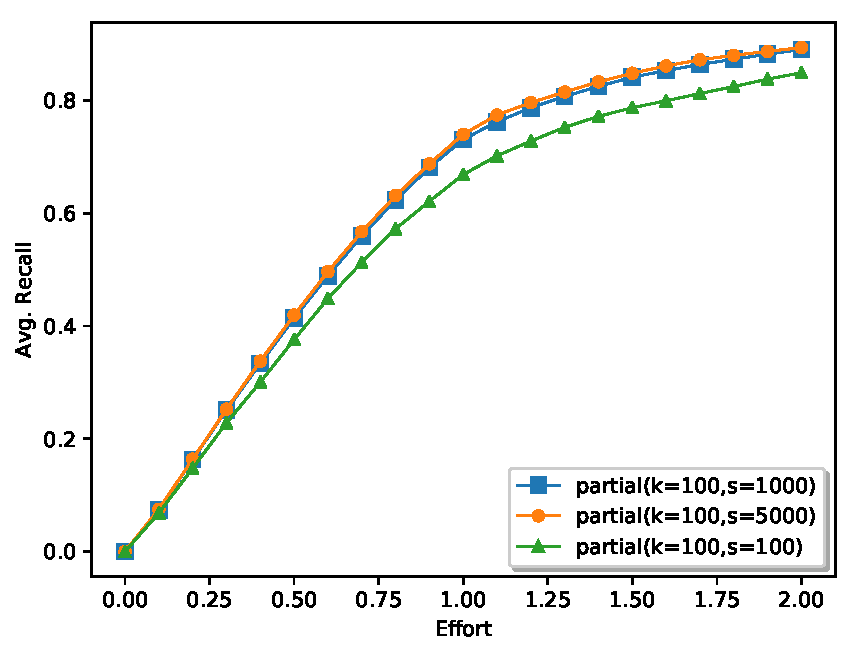
\includegraphics[width=\textwidth]{plots/partial2.pdf}
        \caption{Effect of partial set size on effectiveness. We observe that
        increasing the partial set size beyond 1000 doesn't have any benefit.}
        \label{plot:partial2}
    \end{subfigure}
    ~
    \begin{subfigure}[t]{0.48\textwidth}
        \centering
        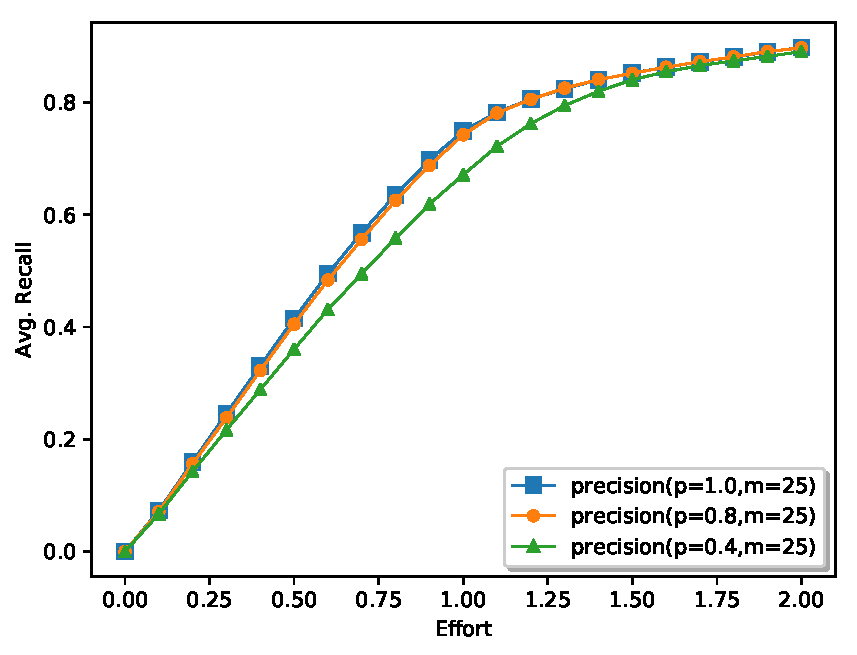
\includegraphics[width=\textwidth]{plots/precision.pdf}
        \caption{Comparison of various settings in \texttt{precision}.}
        \label{plot:prec}
    \end{subfigure}
    \caption{Comparison of various refresh strategies}
\end{figure}


\subsection*{Precision Based Refreshing}

Figure~\ref{plot:prec} compares the gain curves for
various settings of \texttt{precision}.

In this strategy, we fixed \texttt{m=25} and varied \texttt{p}. For
\texttt{p=0.8} and \texttt{p=1.0}, \texttt{precision} achieves $0.75$ recall at
$E_{norm} = 1$ which is similar to \texttt{static(k=1)}. This
similarity of recall is also seen at $E_{norm} = 1.5$ and $E_{norm} = 2$. For
\texttt{precision(p=1.0)}, CAL refreshes whenever a non-relevant judgment
is made, thus behaving very similar to \texttt{static(k=1)}. For
smaller values of \texttt{p}, we observe lower recall values during the initial stages; 
$0.728$ and $0.679$ recall at $E_{norm} = 1$ for \texttt{precision(p=0.6)} and
\texttt{precision(p=0.4)}, respectively. However, they catch up to
\texttt{static(k=1)} at higher $E_{norm}$, as relevant documents
become rarer; $0.853$ and $0.844$ recall at $E_{norm} = 1.5$ for
\texttt{precision(p=0.6)} and \texttt{precision(p=0.4)}, respectively.

This strategy improved the running time of simulations by $42.15\%$
on average when compared to \texttt{static(k=1)}.
\texttt{precision} strategies triggers lower number of refreshes during the
beginning of the CAL process when relevant documents are easier to find. During
the later stages when the relevant documents are harder to find,
\texttt{precision} strategies tend to keep refreshing after every judgment.
Figure~\ref{plot:prec2} compares the \texttt{precision} strategies with
\texttt{static(k=1)} based on how many refreshes were performed to achieve a
certain recall. The \texttt{precision} strategies find a lot of relevant
documents initially since they are easy to find and the precision of CAL's
output is high. \texttt{static(k=1)} keeps refreshing steadily irrespective of
the output quality. As relevant documents become harder to find, we find that
the \texttt{precision} strategies start refreshing as frequently as
\texttt{static(k=1)}.

\begin{figure}
    \centering
    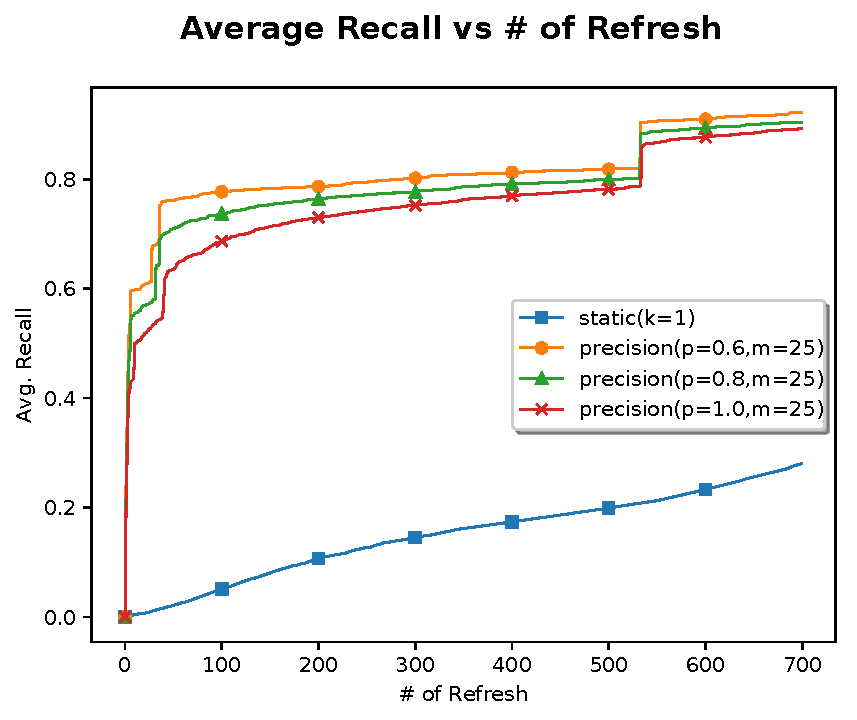
\includegraphics[width=0.6\textwidth]{plots/prec2.pdf}
    \caption{Number of refreshes required to achieve a certain recall $-$
    \texttt{athome1}}
    \label{plot:prec2}
\end{figure}


\subsection*{Effect of Training Iterations}

In all the previously discussed strategies, the improvement in running time over
\texttt{static(k=1)} is either due to refreshing less often (\texttt{exponential},
\texttt{precision}) or by optimizing scoring during a refresh
(\texttt{partial}). The running time of scoring can be further improved by just
increasing the number of threads. However, training is another expensive step
which cannot be trivially distributed across multiple threads. One way to
dramatically reduce the training time is by simply reducing the number of
training iterations (\texttt{it}). In our experiments, the average time to train a classifier
for 100000 (default), 10000, and 1000 number of iterations was 265ms, 33ms, and
4ms respectively.

Despite these massive improvements in the running time, reducing the number of
iterations \texttt{it} beyond a certain point will directly
reduces the quality of the classifier, and thus harming the effectiveness of
CAL. Figure~\ref{plot:train} shows the impact of \texttt{it} on the gain curves
of \texttt{static(k=1)}. We find that reducing \texttt{it} from 100000 to 10000
didn't do any noticeable affect on the recall. This suggests that setting
\texttt{it=10000} for all our experiments might have been enough for the
classifier to converge. Beyond this, we observe noticeable loss in performance.

\begin{figure}
    \centering
    \begin{subfigure}[b]{0.48\textwidth}
        \centering
        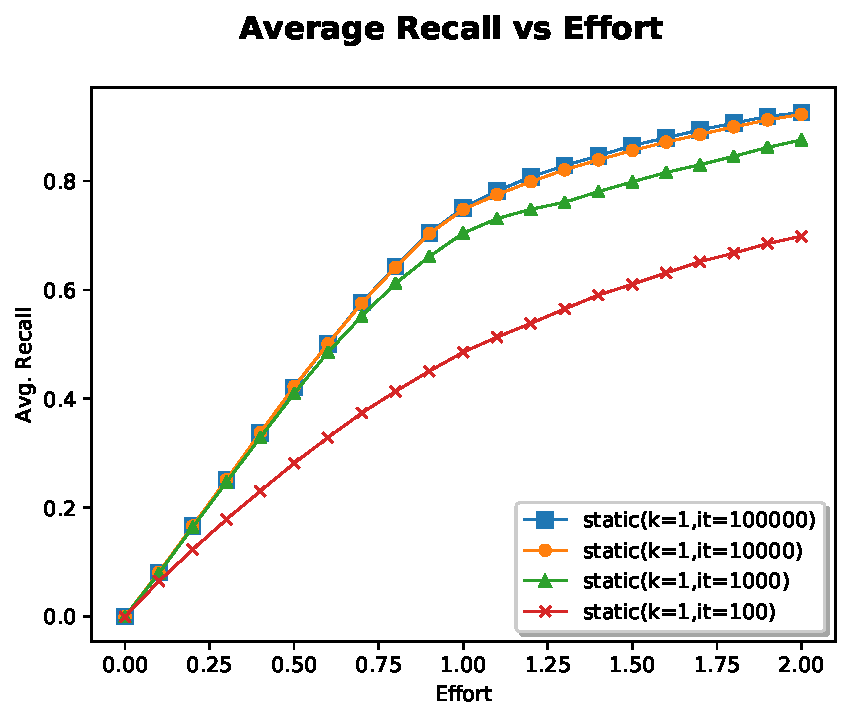
\includegraphics[width=\textwidth]{plots/training.pdf}
        \caption{Effect of number of training iterations on recall}
        \label{plot:train}
    \end{subfigure}
    ~
    \begin{subfigure}[b]{0.48\textwidth}
        \centering
        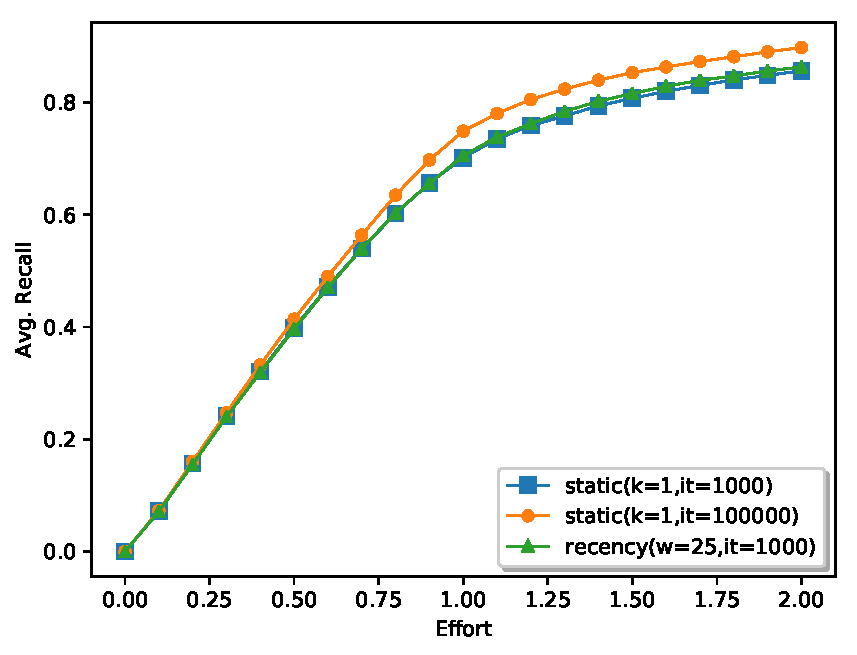
\includegraphics[width=\textwidth]{plots/recency.pdf}
        \caption{Effect of recency weighting on settings with low number of
        training iterations}
        \label{plot:recency}
    \end{subfigure}
    \caption{Gain curves comparing the effect of training iterations and recency
    weighting}
\end{figure}

\begin{table}[]
\centering
\caption{Summary of results for recency weighting}
\label{table.recency}
\resizebox{\textwidth}{!}{%
\begin{tabular}{|c|c|c|c|c|c|}
\hline
\textbf{Strategy} & \begin{tabular}[x]{@{}c@{}}
    \textbf{Avg. Recall}\\ \textbf{@($E_{norm}$=1)}
\end{tabular} & \begin{tabular}[x]{@{}c@{}}
\textbf{Avg. Recall}\\ \textbf{@($E_{norm}$=1.5)}
\end{tabular} & \begin{tabular}[x]{@{}c@{}}
\textbf{Avg. Recall}\\ \textbf{@($E_{norm}$=2)}
\end{tabular} & \begin{tabular}[x]{@{}c@{}}
\textbf{$E_{norm}$ for}\\ \textbf{75\% recall}
\end{tabular}&
\begin{tabular}[x]{@{}c@{}}
    \textbf{Running Time}\\ \textbf{(in min)}
\end{tabular} \\ \hline \hline
\texttt{recency(w=1,it=1000)} & 0.708 & 0.810 & 0.859 & 2.517 & 15.51 \\ \hline
\texttt{recency(w=5,it=1000)} & 0.715 & 0.817 & 0.865 & 2.515 & 16.73 \\ \hline
\texttt{recency(w=10,it=1000)} & 0.713 & 0.817 & 0.867 & 2.483 & 15.99 \\ \hline
\texttt{recency(w=25,it=1000)} & 0.712 & 0.819 & 0.866 & 2.513 & 16.05 \\ \hline
\end{tabular}
}
\end{table}


\subsection*{Recency Weighting}

During our initial experiments, recency weighting seemed to have no
impact on the recall. By reducing the number of training iterations
to $1000$, we introduced significant degradation in the system's effectiveness.
Reducing the number of training iterations also
reduced the running time of simulation by $54.64\%$ when compared to
\texttt{static(k=1)}. We used recency weighting to recover
the lost effectiveness.  \texttt{recency(w=1,it=1000)} is equivalent to
\texttt{static(k=1,it=1000)} and it achieves $0.708$ and $0.810$
recall when $E_{norm}$ is equal to $1$ and $1.5$ respectively. For
$w > 1$, we observe a negligible increase in recall. Moreover,
the recall is consistently lower when compared to
\texttt{static(k=1,it=100000)}. For example, \texttt{recency(w=10,it=1000)} is
only able to achieve $0.817$ recall at $E_{norm}=1.5$, while
\texttt{static(k=1,it=100000)} achieves $0.856$ recall at the same effort.
Table~\ref{table.recency} reports the effectiveness and efficiency measures
averaged over all the datasets.
Table~\ref{table.recency_athome1}-\ref{table.recency_athome4} reports the effectiveness and efficiency measures
for individual datasets.

\newpage
\begin{table}[]
\centering
\caption{Summary of results for \texttt{bmi\_refresh}, \texttt{static\_batch},
    \texttt{partial\_refresh} and \texttt{precision\_strategy} $-$
\texttt{athome1} collection}
\label{table.summary_athome1}
\resizebox{\textwidth}{!}{%
\begin{tabular}{|c|c|c|c|c|c|}
\hline
\textbf{Strategy} & \begin{tabular}[x]{@{}c@{}}
    \textbf{Avg. Recall}\\ \textbf{@($E_{norm}$=1)}
\end{tabular} & \begin{tabular}[x]{@{}c@{}}
\textbf{Avg. Recall}\\ \textbf{@($E_{norm}$=1.5)}
\end{tabular} & \begin{tabular}[x]{@{}c@{}}
\textbf{Avg. Recall}\\ \textbf{@($E_{norm}$=2)}
\end{tabular} & \begin{tabular}[x]{@{}c@{}}
\textbf{$E_{norm}$ for}\\ \textbf{75\% recall}
\end{tabular}&
\begin{tabular}[x]{@{}c@{}}
    \textbf{Running Time}\\ \textbf{(in min)}
\end{tabular} \\ \hline \hline
\texttt{exponential} & 0.718 & 0.826 & 0.904 & 1.150 & 0.30 \\ \hline \hline
\texttt{static(k=1)} & 0.751 & 0.865 & 0.925 & 1.041 & 59.59 \\ \hline
\texttt{static(k=100)} & 0.705 & 0.806 & 0.887 & 1.202 & 0.59 \\ \hline
\hline
\texttt{partial(k=10,s=1000)} & 0.753 & 0.863 & 0.926 & 1.032 & 38.72 \\ \hline
\texttt{partial(k=100,s=500)} & 0.753 & 0.855 & 0.923 & 1.050 & 36.62 \\ \hline
\texttt{partial(k=100,s=1000)} & 0.754 & 0.856 & 0.922 & 1.038 & 36.52 \\ \hline
\texttt{partial(k=100,s=5000)} & 0.756 & 0.855 & 0.921 & 1.049 & 37.19 \\ \hline
\texttt{partial(k=500,s=1000)} & 0.701 & 0.785 & 0.815 & 1.343 & 35.77 \\ \hline
\hline
\texttt{precision(p=0.4,m=25)} & 0.700 & 0.849 & 0.917 & 1.153 & 35.16 \\ \hline
\texttt{precision(p=0.6,m=25)} & 0.735 & 0.860 & 0.923 & 1.087 & 39.44 \\ \hline
\texttt{precision(p=0.8,m=25)} & 0.749 & 0.862 & 0.927 & 1.047 & 35.52 \\ \hline
\texttt{precision(p=1.0,m=25)} & 0.753 & 0.864 & 0.927 & 1.034 & 36.96 \\ \hline
\end{tabular}
}
\end{table}

\begin{table}[]
\centering
\caption{Summary of results for \texttt{bmi\_refresh}, \texttt{static\_batch},
    \texttt{partial\_refresh} and \texttt{precision\_strategy} $-$
\texttt{athome2} collection}
\label{table.summary_athome2}
\resizebox{\textwidth}{!}{%
\begin{tabular}{|c|c|c|c|c|c|}
\hline
\textbf{Strategy} & \begin{tabular}[x]{@{}c@{}}
    \textbf{Avg. Recall}\\ \textbf{@($E_{norm}$=1)}
\end{tabular} & \begin{tabular}[x]{@{}c@{}}
\textbf{Avg. Recall}\\ \textbf{@($E_{norm}$=1.5)}
\end{tabular} & \begin{tabular}[x]{@{}c@{}}
\textbf{Avg. Recall}\\ \textbf{@($E_{norm}$=2)}
\end{tabular} & \begin{tabular}[x]{@{}c@{}}
\textbf{$E_{norm}$ for}\\ \textbf{75\% recall}
\end{tabular}&
\begin{tabular}[x]{@{}c@{}}
    \textbf{Running Time}\\ \textbf{(in min)}
\end{tabular} \\ \hline \hline
\texttt{exponential} & 0.679 & 0.801 & 0.861 & 1.467 & 0.23 \\ \hline \hline
\texttt{static(k=1)} & 0.685 & 0.809 & 0.862 & 1.470 & 28.88 \\ \hline
\texttt{static(k=100)} & 0.637 & 0.778 & 0.848 & 1.594 & 0.29 \\ \hline
\hline
\texttt{partial(k=10,s=1000)} & 0.686 & 0.809 & 0.862 & 1.458 & 12.08 \\ \hline
\texttt{partial(k=100,s=500)} & 0.669 & 0.806 & 0.861 & 1.485 & 9.74 \\ \hline
\texttt{partial(k=100,s=1000)} & 0.681 & 0.808 & 0.861 & 1.460 & 10.39 \\ \hline
\texttt{partial(k=100,s=5000)} & 0.686 & 0.810 & 0.861 & 1.462 & 12.10 \\ \hline
\texttt{partial(k=500,s=1000)} & 0.614 & 0.726 & 0.784 & 1.932 & 9.69 \\ \hline
\hline
\texttt{precision(p=0.4,m=25)} & 0.657 & 0.807 & 0.861 & 1.505 & 12.64 \\ \hline
\texttt{precision(p=0.6,m=25)} & 0.683 & 0.809 & 0.863 & 1.467 & 15.02 \\ \hline
\texttt{precision(p=0.8,m=25)} & 0.690 & 0.811 & 0.862 & 1.450 & 16.65 \\ \hline
\texttt{precision(p=1.0,m=25)} & 0.690 & 0.810 & 0.861 & 1.445 & 17.41 \\ \hline
\end{tabular}
}
\end{table}

\begin{table}[]
\centering
\caption{Summary of results for \texttt{bmi\_refresh}, \texttt{static\_batch},
    \texttt{partial\_refresh} and \texttt{precision\_strategy} $-$
\texttt{athome3} collection}
\label{table.summary_athome3}
\resizebox{\textwidth}{!}{%
\begin{tabular}{|c|c|c|c|c|c|}
\hline
\textbf{Strategy} & \begin{tabular}[x]{@{}c@{}}
    \textbf{Avg. Recall}\\ \textbf{@($E_{norm}$=1)}
\end{tabular} & \begin{tabular}[x]{@{}c@{}}
\textbf{Avg. Recall}\\ \textbf{@($E_{norm}$=1.5)}
\end{tabular} & \begin{tabular}[x]{@{}c@{}}
\textbf{Avg. Recall}\\ \textbf{@($E_{norm}$=2)}
\end{tabular} & \begin{tabular}[x]{@{}c@{}}
\textbf{$E_{norm}$ for}\\ \textbf{75\% recall}
\end{tabular}&
\begin{tabular}[x]{@{}c@{}}
    \textbf{Running Time}\\ \textbf{(in min)}
\end{tabular} \\ \hline \hline
\texttt{exponential} & 0.783 & 0.862 & 0.887 & 4.610 & 0.60 \\ \hline \hline
\texttt{static(k=1)} & 0.827 & 0.878 & 0.899 & 4.266 & 32.45 \\ \hline
\texttt{static(k=100)} & 0.614 & 0.719 & 0.789 & 5.288 & 0.33 \\ \hline
\hline
\texttt{partial(k=10,s=1000)} & 0.818 & 0.878 & 0.895 & 4.270 & 11.99 \\ \hline
\texttt{partial(k=100,s=500)} & 0.769 & 0.848 & 0.889 & 4.317 & 10.51 \\ \hline
\texttt{partial(k=100,s=1000)} & 0.776 & 0.858 & 0.891 & 4.324 & 9.86 \\ \hline
\texttt{partial(k=100,s=5000)} & 0.800 & 0.877 & 0.899 & 4.157 & 10.72 \\ \hline
\texttt{partial(k=500,s=1000)} & 0.742 & 0.783 & 0.800 & 5.384 & 9.44 \\ \hline
\hline
\texttt{precision(p=0.4,m=25)} & 0.675 & 0.869 & 0.888 & 4.460 & 16.24 \\ \hline
\texttt{precision(p=0.6,m=25)} & 0.774 & 0.875 & 0.894 & 4.545 & 18.32 \\ \hline
\texttt{precision(p=0.8,m=25)} & 0.813 & 0.877 & 0.899 & 4.363 & 19.44 \\ \hline
\texttt{precision(p=1.0,m=25)} & 0.831 & 0.878 & 0.902 & 4.264 & 20.12 \\ \hline
\end{tabular}
}
\end{table}

\begin{table}[]
\centering
\caption{Summary of results for \texttt{bmi\_refresh}, \texttt{static\_batch},
    \texttt{partial\_refresh} and \texttt{precision\_strategy} $-$
\texttt{athome4} collection}
\label{table.summary_athome4}
\resizebox{\textwidth}{!}{%
\begin{tabular}{|c|c|c|c|c|c|}
\hline
\textbf{Strategy} & \begin{tabular}[x]{@{}c@{}}
    \textbf{Avg. Recall}\\ \textbf{@($E_{norm}$=1)}
\end{tabular} & \begin{tabular}[x]{@{}c@{}}
\textbf{Avg. Recall}\\ \textbf{@($E_{norm}$=1.5)}
\end{tabular} & \begin{tabular}[x]{@{}c@{}}
\textbf{Avg. Recall}\\ \textbf{@($E_{norm}$=2)}
\end{tabular} & \begin{tabular}[x]{@{}c@{}}
\textbf{$E_{norm}$ for}\\ \textbf{75\% recall}
\end{tabular}&
\begin{tabular}[x]{@{}c@{}}
    \textbf{Running Time}\\ \textbf{(in min)}
\end{tabular} \\ \hline \hline
\texttt{exponential} & 0.713 & 0.839 & 0.894 & 1.414 & 0.19 \\ \hline \hline
\texttt{static(k=1)} & 0.754 & 0.872 & 0.913 & 1.211 & 15.85 \\ \hline
\texttt{static(k=100)} & 0.651 & 0.772 & 0.837 & 1.759 & 0.15 \\ \hline
\hline
\texttt{partial(k=10,s=1000)} & 0.754 & 0.871 & 0.913 & 1.214 & 10.07 \\ \hline
\texttt{partial(k=100,s=500)} & 0.733 & 0.847 & 0.898 & 1.275 & 9.16 \\ \hline
\texttt{partial(k=100,s=1000)} & 0.739 & 0.855 & 0.899 & 1.276 & 9.50 \\ \hline
\texttt{partial(k=100,s=5000)} & 0.746 & 0.864 & 0.903 & 1.262 & 9.34 \\ \hline
\texttt{partial(k=500,s=1000)} & 0.687 & 0.785 & 0.818 & 2.588 & 9.47 \\ \hline
\hline
\texttt{precision(p=0.4,m=25)} & 0.684 & 0.850 & 0.902 & 1.348 & 6.48 \\ \hline
\texttt{precision(p=0.6,m=25)} & 0.721 & 0.867 & 0.909 & 1.285 & 8.09 \\ \hline
\texttt{precision(p=0.8,m=25)} & 0.745 & 0.870 & 0.910 & 1.235 & 9.36 \\ \hline
\texttt{precision(p=1.0,m=25)} & 0.747 & 0.869 & 0.909 & 1.225 & 9.60 \\ \hline
\end{tabular}
}
\end{table}

\begin{table}[]
\centering
\caption{Summary of results for recency weighting $-$ \texttt{athome1}}
\label{table.recency_athome1}
\resizebox{\textwidth}{!}{%
\begin{tabular}{|c|c|c|c|c|c|}
\hline
\textbf{Strategy} & \begin{tabular}[x]{@{}c@{}}
    \textbf{Avg. Recall}\\ \textbf{@($E_{norm}$=1)}
\end{tabular} & \begin{tabular}[x]{@{}c@{}}
\textbf{Avg. Recall}\\ \textbf{@($E_{norm}$=1.5)}
\end{tabular} & \begin{tabular}[x]{@{}c@{}}
\textbf{Avg. Recall}\\ \textbf{@($E_{norm}$=2)}
\end{tabular} & \begin{tabular}[x]{@{}c@{}}
\textbf{$E_{norm}$ for}\\ \textbf{75\% recall}
\end{tabular}&
\begin{tabular}[x]{@{}c@{}}
    \textbf{Running Time}\\ \textbf{(in min)}
\end{tabular} \\ \hline \hline
\texttt{recency(w=1,it=1000)} & 0.704 & 0.797 & 0.875 & 1.287 & 22.07 \\ \hline
\texttt{recency(w=5,it=1000)} & 0.705 & 0.813 & 0.887 & 1.233 & 26.71 \\ \hline
\texttt{recency(w=10,it=1000)} & 0.708 & 0.824 & 0.891 & 1.233 & 23.30 \\ \hline
\texttt{recency(w=25,it=1000)} & 0.708 & 0.827 & 0.893 & 1.228 & 23.15 \\ \hline
\end{tabular}
}
\end{table}

\begin{table}[]
\centering
\caption{Summary of results for recency weighting $-$ \texttt{athome2}}
\label{table.recency_athome2}
\resizebox{\textwidth}{!}{%
\begin{tabular}{|c|c|c|c|c|c|}
\hline
\textbf{Strategy} & \begin{tabular}[x]{@{}c@{}}
    \textbf{Avg. Recall}\\ \textbf{@($E_{norm}$=1)}
\end{tabular} & \begin{tabular}[x]{@{}c@{}}
\textbf{Avg. Recall}\\ \textbf{@($E_{norm}$=1.5)}
\end{tabular} & \begin{tabular}[x]{@{}c@{}}
\textbf{Avg. Recall}\\ \textbf{@($E_{norm}$=2)}
\end{tabular} & \begin{tabular}[x]{@{}c@{}}
\textbf{$E_{norm}$ for}\\ \textbf{75\% recall}
\end{tabular}&
\begin{tabular}[x]{@{}c@{}}
    \textbf{Running Time}\\ \textbf{(in min)}
\end{tabular} \\ \hline \hline
\texttt{recency(w=1,it=1000)} & 0.630 & 0.749 & 0.806 & 1.895 & 15.36 \\ \hline
\texttt{recency(w=5,it=1000)} & 0.631 & 0.751 & 0.810 & 1.846 & 15.70 \\ \hline
\texttt{recency(w=10,it=1000)} & 0.633 & 0.751 & 0.812 & 1.824 & 15.46 \\ \hline
\texttt{recency(w=25,it=1000)} & 0.633 & 0.752 & 0.809 & 1.854 & 15.97 \\ \hline
\end{tabular}
}
\end{table}

\begin{table}[]
\centering
\caption{Summary of results for recency weighting $-$ \texttt{athome3}}
\label{table.recency_athome3}
\resizebox{\textwidth}{!}{%
\begin{tabular}{|c|c|c|c|c|c|}
\hline
\textbf{Strategy} & \begin{tabular}[x]{@{}c@{}}
    \textbf{Avg. Recall}\\ \textbf{@($E_{norm}$=1)}
\end{tabular} & \begin{tabular}[x]{@{}c@{}}
\textbf{Avg. Recall}\\ \textbf{@($E_{norm}$=1.5)}
\end{tabular} & \begin{tabular}[x]{@{}c@{}}
\textbf{Avg. Recall}\\ \textbf{@($E_{norm}$=2)}
\end{tabular} & \begin{tabular}[x]{@{}c@{}}
\textbf{$E_{norm}$ for}\\ \textbf{75\% recall}
\end{tabular}&
\begin{tabular}[x]{@{}c@{}}
    \textbf{Running Time}\\ \textbf{(in min)}
\end{tabular} \\ \hline \hline
\texttt{recency(w=1,it=1000)} & 0.791 & 0.866 & 0.875 & 5.316 & 19.00 \\ \hline
\texttt{recency(w=5,it=1000)} & 0.808 & 0.869 & 0.880 & 5.435 & 18.87 \\ \hline
\texttt{recency(w=10,it=1000)} & 0.799 & 0.862 & 0.881 & 5.439 & 19.54 \\ \hline
\texttt{recency(w=25,it=1000)} & 0.800 & 0.864 & 0.879 & 5.450 & 19.52 \\ \hline
\end{tabular}
}
\end{table}

\begin{table}[]
\centering
\caption{Summary of results for recency weighting $-$ \texttt{athome4}}
\label{table.recency_athome4}
\resizebox{\textwidth}{!}{%
\begin{tabular}{|c|c|c|c|c|c|}
\hline
\textbf{Strategy} & \begin{tabular}[x]{@{}c@{}}
    \textbf{Avg. Recall}\\ \textbf{@($E_{norm}$=1)}
\end{tabular} & \begin{tabular}[x]{@{}c@{}}
\textbf{Avg. Recall}\\ \textbf{@($E_{norm}$=1.5)}
\end{tabular} & \begin{tabular}[x]{@{}c@{}}
\textbf{Avg. Recall}\\ \textbf{@($E_{norm}$=2)}
\end{tabular} & \begin{tabular}[x]{@{}c@{}}
\textbf{$E_{norm}$ for}\\ \textbf{75\% recall}
\end{tabular}&
\begin{tabular}[x]{@{}c@{}}
    \textbf{Running Time}\\ \textbf{(in min)}
\end{tabular} \\ \hline \hline
\texttt{recency(w=1,it=1000)} & 0.709 & 0.830 & 0.881 & 1.570 & 5.59 \\ \hline
\texttt{recency(w=5,it=1000)} & 0.715 & 0.834 & 0.883 & 1.544 & 5.63 \\ \hline
\texttt{recency(w=10,it=1000)} & 0.711 & 0.831 & 0.885 & 1.434 & 5.65 \\ \hline
\texttt{recency(w=25,it=1000)} & 0.707 & 0.834 & 0.882 & 1.522 & 5.58 \\ \hline
\end{tabular}
}
\end{table}
